\chapter{热传导方程}
\intro{本章建立热传导方程，讨论初值问题和半无界问题的解法。}

\begin{mydefinition}{热传导方程}
温度分布 $u(x,t)$ 满足：
\[
\frac{\partial u}{\partial t}=k\lapl u+f(\vect{x},t)
\]
其中 $k$ 为热扩散系数，$f$ 为内热源项。
\end{mydefinition}

\section{基本解}

\begin{theorem}[热核]
三维热传导方程的基本解：
\[
\Phi(\vect{x},t)=\frac{1}{(4\pi kt)^{3/2}}\exp\left(-\frac{|\vect{x}|^2}{4kt}\right),\quad t>0
\]
\end{theorem}

\section{初值问题}

\begin{mydefinition}{一维初值问题的解}
\[
u(x,t)=\int_{-\infty}^{+\infty}\Phi(x-\xi,t)\phi(\xi)\,d\xi
\]
\end{mydefinition}

\begin{figure}[htbp]
\centering
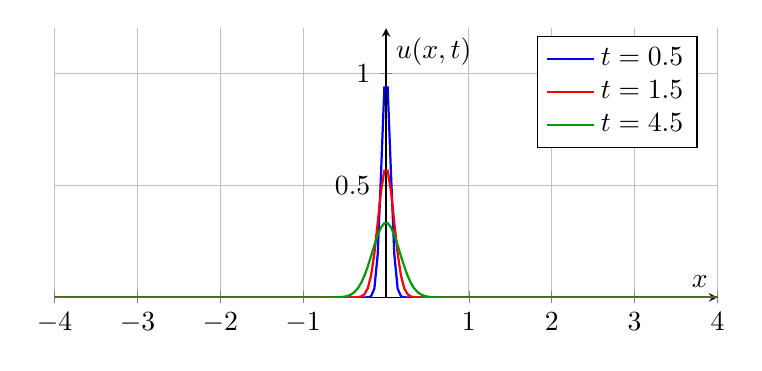
\begin{tikzpicture}
\begin{axis}[
	axis lines=middle,
	xlabel=$x$,
	ylabel={$u(x,t)$},
	xmin=-4,xmax=4,
	ymin=0,ymax=1.2,
	legend pos=north east,
	grid=major,
	width=10cm,height=5cm,
]
\addplot[blue,thick,domain=-4:4,samples=200]{exp(-deg(x)^2/20)};
\addplot[red,thick,domain=-4:4,samples=200]{exp(-deg(x)^2/60)/sqrt(3)};
\addplot[green!60!black,thick,domain=-4:4,samples=200]{exp(-deg(x)^2/180)/3};
\legend{$t=0.5$,$t=1.5$,$t=4.5$}
\end{axis}
\end{tikzpicture}
\caption{热传导方程解的扩散}
\end{figure}

\section{半无界问题}

\begin{theorem}[镜像法]
半无界问题（$x>0$）通过延拓初始条件求解：Dirichlet 条件奇延拓，Neumann 条件偶延拓。
\end{theorem}

\begin{remark}
热传导方程的解具有\textbf{无穷传播速度}：即使初始温度分布紧支集，对任意 $t>0$，解在整个空间上非零。这与波动方程的有限传播速度形成对比。
\end{remark}
